\documentclass[a4paper]{article}
\usepackage[utf8]{inputenc}
\usepackage[english]{babel}
\usepackage{hyperref}
\usepackage{url}
\usepackage{enumerate}
\usepackage{subfiles}
\usepackage[lmargin=3cm,rmargin=3cm,tmargin=2.5cm,bmargin=2.5cm]{geometry}
\usepackage{titlesec}
\usepackage{todonotes}
\usepackage{graphicx}
\usepackage{parskip}
\usepackage{minted}

\definecolor{linkcol}{RGB}{42, 93, 176}
\definecolor{monokaibg} {RGB} {41, 42, 35}

\setminted{linenos=false, breaklines, breakanywhere, numbersep=5pt, framesep=2pt, autogobble, xleftmargin=10pt, xrightmargin=27pt, fontsize=\footnotesize, bgcolor=monokaibg}
\usemintedstyle{monokai}

%Package setup
\hypersetup{
colorlinks=true,
linktoc=all,
linkcolor=black,
citecolor=magenta,
urlcolor=linkcol,
}


\title{HazzardHulen.io\\[4cm]
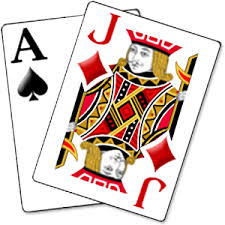
\includegraphics[width=.7\textwidth]{blackjack}
\vfill}
\author{
  Anders Bundgaard\\
  \texttt{abund14@student.sdu.dk}
  \and
  Casper Beese Nielsen\\
  \texttt{casni14@student.sdu.dk}
  \and
  Oliver Vestergaard\\
  \texttt{olves13@student.sdu.dk}
  \and
  Simon Hjortshøj Larsen\\
  \texttt{sila114@student.sdu.dk}
  \and
  Steen Schütt\\
  \texttt{stesc14@student.sdu.dk}
  \and
  Thomas Lemqvist\\
  \texttt{thlem14@student.sdu.dk}
}

\begin{document}
\maketitle
\newpage
\tableofcontents
\newpage


\section{The Software}
HazardHulen.io is a multiplayer blackjack table, where players can bet virtual
currency to participate in a round of blackjack. The game uses the same ruleset
as regular blackjack played in casinos, with a few details left out for
simplicity.
Players play against an artificial intelligence which acts as the dealer, and
win double their bet if they beat the AI. If a player loses, his bet is lost.
All players get a set amount of virtual money when they join the table, and have
to place a bet of at least a minimum amount to play. If a player does not place
a bet within a certain time period in between rounds, he is labeled as inactive,
and cannot take part in the next round.
\section{Technology}
This section describes the technologies used to implement this system.
\subsection{Client Side}
The client is written in \textit{HTML} and \textit{jQuery}, which uses \textit{socket.io}, which is
a web socket library, to connect to the server.
\subsection{Server Side}
The server is written in \textit{JavaScript} and uses \textit{socket.io} to communicate with
the clients.

The server utilizes the duplex connection, provided by \textit{socket.io} to
synchronize the state of the game across all clients


\section{UML Sequence Diagram}
\begin{figure}[H]
  \centering
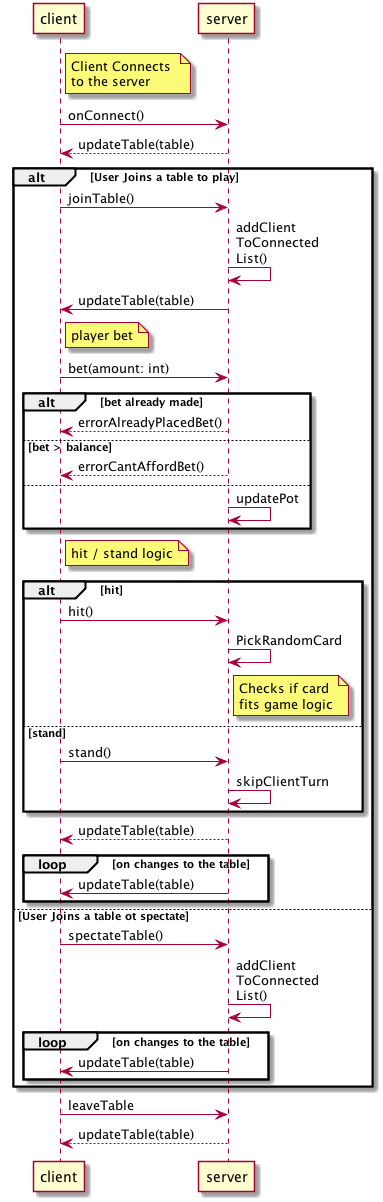
\includegraphics[height=\textheight]{sequence}
\end{figure}

The sequence diagram, shown above, shows all calls made between the server and the client.

The server is responsible for synchronizing the table across all clients.
It uses the table object \textit{(as seen in the object diagram below)} for this, in the updateTable method.

\section{UML Object Diagram}
\begin{figure}[hbt]
  \centering
  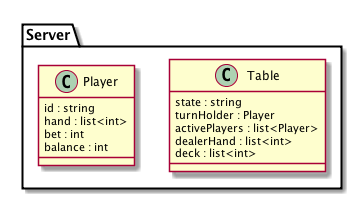
\includegraphics{ClassDiag}
\end{figure}
The object diagram contains the two key objects used in this project, \textit{Table}
and \textit{Player}.

* The types set in the fields in the objects, are not according to
UML standards.
\section{Walkthrough of key Code-snippets}
\subsection{The Connection between the client and server}
\begin{listing}[H]
\begin{minted}[firstnumber=1]{javascript}

var express = require('express');
var app = express();
var server = require('http').createServer(app);
var io = require('socket.io')(server);

// ... omitted for brevity

server.listen(13337);

\end{minted}
\end{listing}
The code snippet above is responsible for making the serve serve the clients
the last line, sets the port, on which is listened on for requests to the server.

\begin{listing}[H]
\begin{minted}[firstnumber=1]{javascript}

var port = 13337;

// ... omitted for brevity,

	var socket = io.connect("http://localhost:" + port + "/");

\end{minted}
\end{listing}

The code snippet above is taken from the client, and makes it connect to the server, in this case it connects to the localhost, on the port 13337.


\subsection{The calls from the Client to the Server}
\begin{listing}[H]
\begin{minted}[firstnumber=1]{javascript}

io.on('connection', function (client) {

  // ... omitted for brevity

    client.emit('setId', id);
    client.emit('updateTableState', table);

    client.on('joinTable', function () {

      // ... omitted for brevity

    });

  // ... omitted for brevity

});

\end{minted}
\end{listing}
The code snippet above is taken from the server, and it is responsible for taking commands from the client.

\section{How to Run}
To run the server, you have to have npm (it can be downloaded along with
  node here: \url{https://nodejs.org/en/download/}).

Run the following commands to start the server:
\begin{minted}[firstnumber=1, bgcolor=white]{sh}
	$ npm install
\end{minted}
  
Install bower by running this command, in the command line to install
bower: (from: \url{https://bower.io})

\begin{minted}[firstnumber=1, bgcolor=white]{sh}
	$ npm install -g bower
\end{minted}

To start the server, now you simply just has to run the following command.

\begin{minted}[firstnumber=1, bgcolor=white]{sh}
	$ npm start
\end{minted}

Now the server should be up and running.

To connect a client to the server, go to \url{http://localhost:13337/}

\section{References}
\subsection*{npm packages}
\url{https://nodejs.org/en/download/}\\
\url{https://bower.io}\\
\url{https://lodash.com}\\
\url{http://socket.io}\\
\url{https://www.npmjs.com/package/monolog}\\

\subsection*{Helpful Links}
\url{http://www.programwitherik.com/socket-io-tutorial-with-node-js-and-express/}\\

\subsection*{Information about Blackjack}
\url{https://en.wikipedia.org/wiki/Blackjack}\\
	
\end{document}